\documentclass[tikz, border=10pt]{standalone}
\usepackage{tikz}
\usepackage[sfdefault]{roboto}
\usepackage[T1]{fontenc}
\usetikzlibrary{shapes.misc, positioning, arrows.meta, fit, calc, backgrounds}

\begin{document}

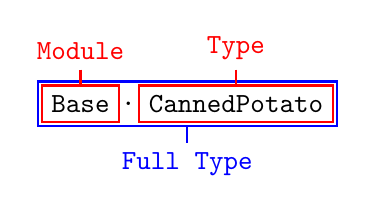
\begin{tikzpicture}[
    node distance=0.3cm,
    box/.style={rectangle, draw, thick},
    func/.style={font=\ttfamily},
    arrow/.style={thick},
    dashed_arrow/.style={-{Latex[length=6pt, width=4pt]}, thick, dashed},
    line/.style={thick},
]

%% NODES
    % original tools
    \node[func] (module) {Base};
    \node[func, right=-0.1cm of module] (dot) {.};
    \node[func, right=0.25cm of module] (type) {CannedPotato};

    \node[func, text=red, above=0.2cm of module] (module_label) {Module};
    \node[func, text=red, above=0.2cm of type] (type_label) {Type};


    \node[box, inner sep=0.00cm, draw=red!100, fit=(module)] (module_box) {};
    \node[box, inner sep=0.00cm, draw=red!100, fit=(type)] (type_box) {};
    \node[box, inner sep=0.05cm, draw=blue!100, fit=(module) (type)] (full_box) {};

    \node[func, text=blue, below=0.2cm of full_box] (full_label) {Full Type};


    \draw[arrow, draw=red!100] (module_label) -- (module);
    \draw[arrow, draw=red!100] (type_label) -- (type);
    \draw[arrow, draw=blue!100] (full_label) -- (full_box);

    
\end{tikzpicture}

\end{document}
